\newpage
\section{Implementierung}
\label{sec:implementierung}


In diesem Kapitel wird die Umsetzung des im vorherigen beschriebenen Konzepts bis zum Punkt der Abgabe erläutert.
Bei dieser Form der Applikation handelt es sich um einen lauffähigen Prototyp, der bisher nicht verlässlich einsetzbar wäre.
Der Fokus der Implementierung lag bei diesem auf der Realisierung der Kernfunktionen zur Verarbeitung, Speicherung und Darstellung der XML-basierten Testberichte.
Der Prototyp bildet damit die grundsätzlichen Funktionsabläufe der geplanten Web-Applikation ab, stellt jedoch noch kein vollständig ausgereiftes Produkt dar.
Die Mängel, nötigen Änderungen und Erweiterungen bis zu einem nutzbaren Produkt werden in den Kapiteln 6 und 7 behandelt.

Die Implementierung erfolgte schrittweise in iterativen Entwicklungszyklen.
Zunächst wurde das Grundgerüst der Flask-Anwendung erstellt, dann die Einlesefunktion erstellt.
Anschließend die Datenbankanbindung und zuletzt die Benutzeroberfläche mit den Auswertungs- und Visualisierungsfunktionen integriert.
Dabei wurde besonderer Wert auf eine modulare Struktur gelegt, um die Erweiterbarkeit des Systems zu gewährleisten.

Die Beschreibung der Implementierung wird hier an Architekturschichten angelehnt, um eine aufeinander aufbauende Erklärung zu schaffen.

\subsection{Programmstruktur}
\label{subsec:programmstruktur}


Im folgenden Abschnitt wird die genaue Struktur des Programmcodes dargestellt, um mit dieser die in den folgenden
Unterkapiteln zu beschreiben und der Gesamtstruktur besser zuordnen zu können.
Die Programmstruktur folgt dem in Unterkapitel ref beschriebenen Strukturmuster.
Eine genaue Beschreibung der Struktur des Programmcodes.
Struktur und der Inhalt der Ordner werden in der folgenden Abbildung \ref{fig: Genaue Struktur des Applikations-Ordners} dargestellt.
Die in der Abbildung vorkommenden Daten entsprechen genau den der Anwendung.


\begin{figure}[H]
    \centering
    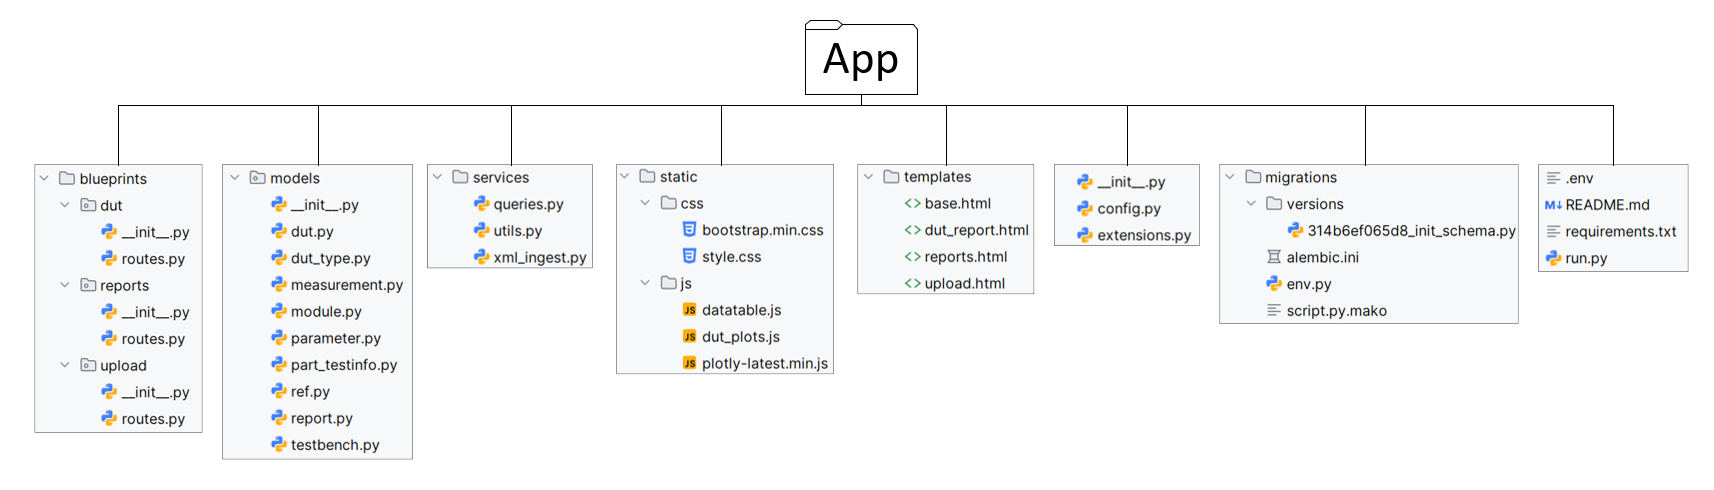
\includegraphics[width=1\textwidth]{Grafiken/Min Ordnerstruktur Projekt.png}
    \caption{Genaue Struktur des Applikations-Ordners}
    \label{fig: Genaue Struktur des Applikations-Ordners}
    {Quelle: Eigene Darstellung mit Microsoft Visio}
\end{figure}
\input{Kapitel/2. Hauptteil/4. Implemetierung/4.1 Entwicklung der Benutzeroberfläche}
\subsection{Einlesen und Verarbeiten von XML-Daten}
\label{subsec:einlesen-und-verarbeiten-von-xml-daten}

Wie bereits im vorherigen Unterkapitel erläutert, beginnt das Einlesen und Verarbeiten mit der Übergabe des Inhaltes aus der
Upload-Seite der Web-Applikation über die Post-Methode.

Die daraus erhaltenen Daten werden in die Funktion \code{upload()} in der Datei \code{route.py} für die Upload-Seite übergeben.
weitergegeben und von der Funktion \code{ingest\_xml()} aus \code{xml\_ingest.py} verarbeitet wird.
Bevor die Daten an \code{ingest\_xml()} übergeben werden, werden diese durch die Funktion \code{parse\_xml\_string()} aus
\code{utils} geparst.
und somit die Struktur der XML-Daten grundlegend überprüft.
Für das Parsen wird die Bibliothek \code{lxml} genutzt.

Die relevanten Daten werden in \code{ingest\_xml()} durch Hilfsfunktionen extrahiert und in Variablen bzw. Listen
vorsortiert und gespeichert.

Die Hilfsfunktionen nutzen hierbei die XPath-Adressierung über die Funktion \code{xpath()} aus der Bibliothek \code{lxml}
bzw. aus dem Modul \code{lxml.etree}, um die relevanten Daten als Listen zurückzugeben.
In Abbildung \ref{fig: Codeausschnitt für die Listenspeicherung mit Hilfsfunktionen} ist zur Veranschaulichung ein Codeabschnitt dargestellt, in den über die Hilfsfunktionen die Variablen
für das Vorsortieren und Speichern befüllt werden.

\begin{figure}[H]
    \centering
    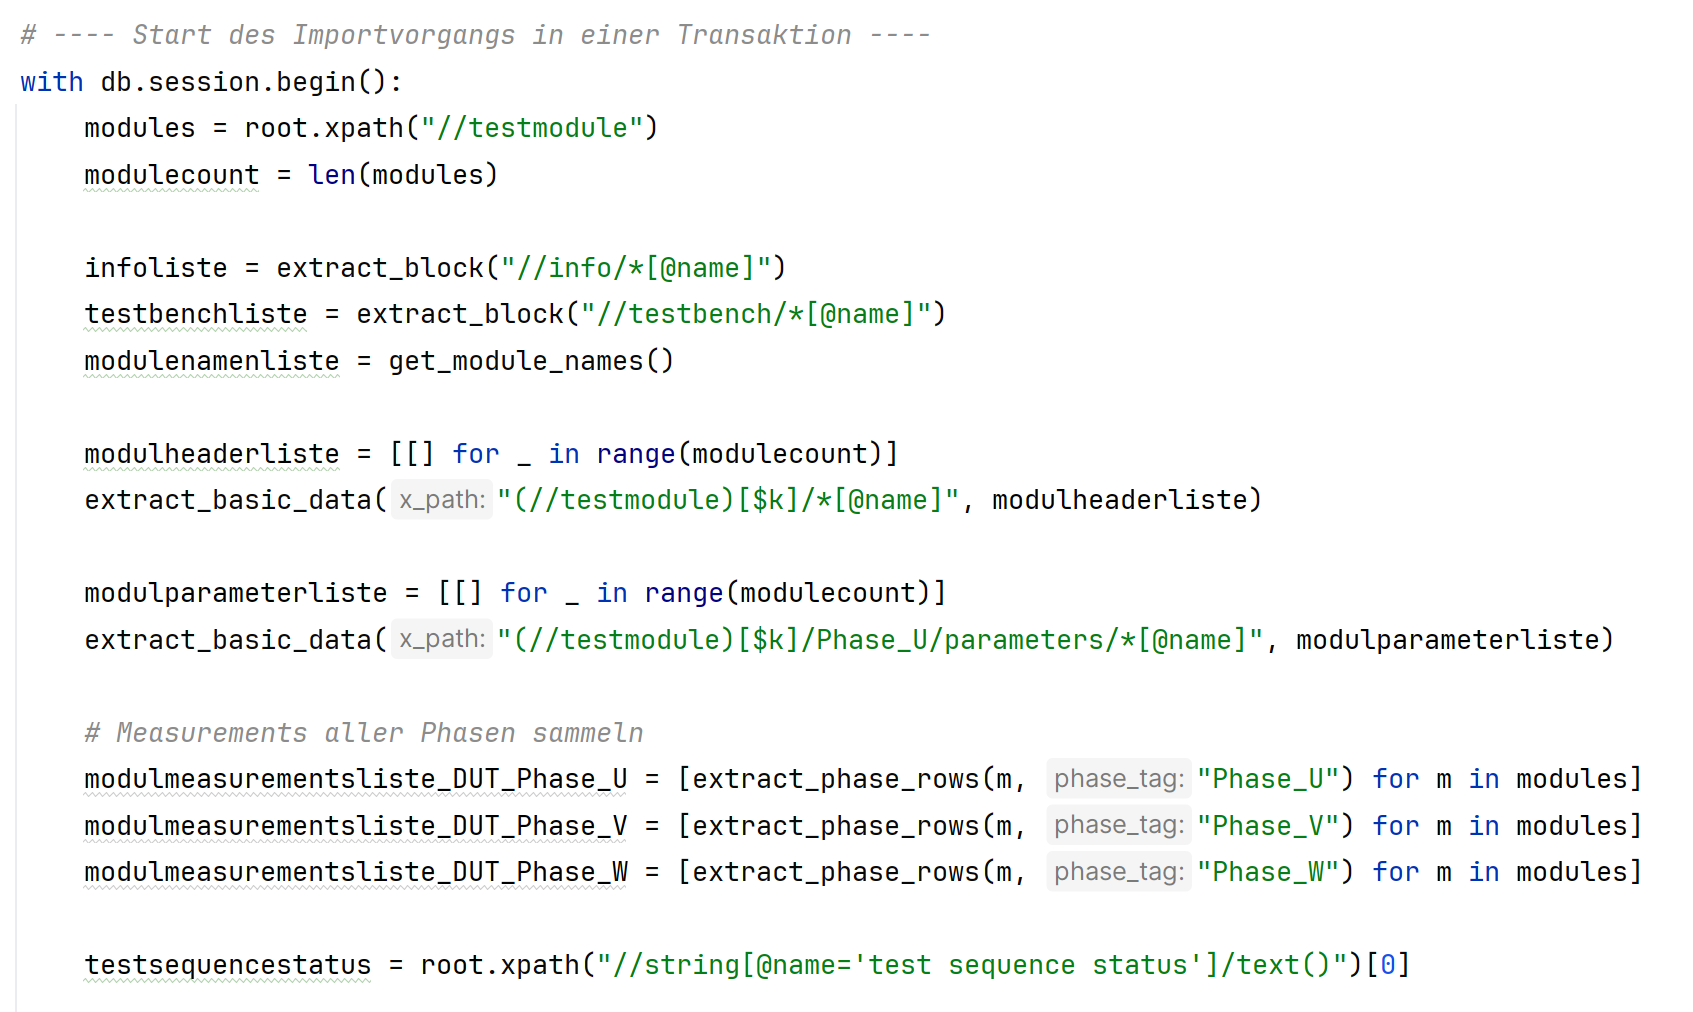
\includegraphics[width=1\textwidth]{Grafiken/5.3 Listen}
    \caption{Codeausschnitt für die Listenspeicherung mit Hilfsfunktionen}
    \label{fig: Codeausschnitt für die Listenspeicherung mit Hilfsfunktionen}
    {Quelle: Eigene Darstellung}
\end{figure}

Nach dem Vorsortieren und Speichern werden \ac{ORM}-Objekte für das Überführen der Daten in die Datenbank erstellt.
Mit Hilfe der Suchfunktion \code{get\_value\_by\_name()} werden die Daten anhand der Namen aus den Namen-Attributen gesucht,
die zusammen mit dem Inhalt aus dem XML-Element in Tupeln gespeichert sind.
den Namen-Attribute, welche zusammen mit dem Inhalt aus dem XML-Element in Tupeln gespeichert sind, aus den Listen gesucht.
Der Inhalt wird zurückgegeben, außer wenn der Name nicht gefunden wird.
Dann wird ein Standardwert zurückgegeben.
Dieser Standardwert löst beim Eintragen in die Datenbank bewusst Fehler aus, um Fehler in der Übertragung und der
Verarbeitung der XML-Daten zu erkennen.
Für den Code zu \code{get\_value\_by\_name() siehe Abbildung \ref{fig: Codeausschnitt für die Suchfunktion in den Listen}.

\begin{figure}[H]
    \centering
    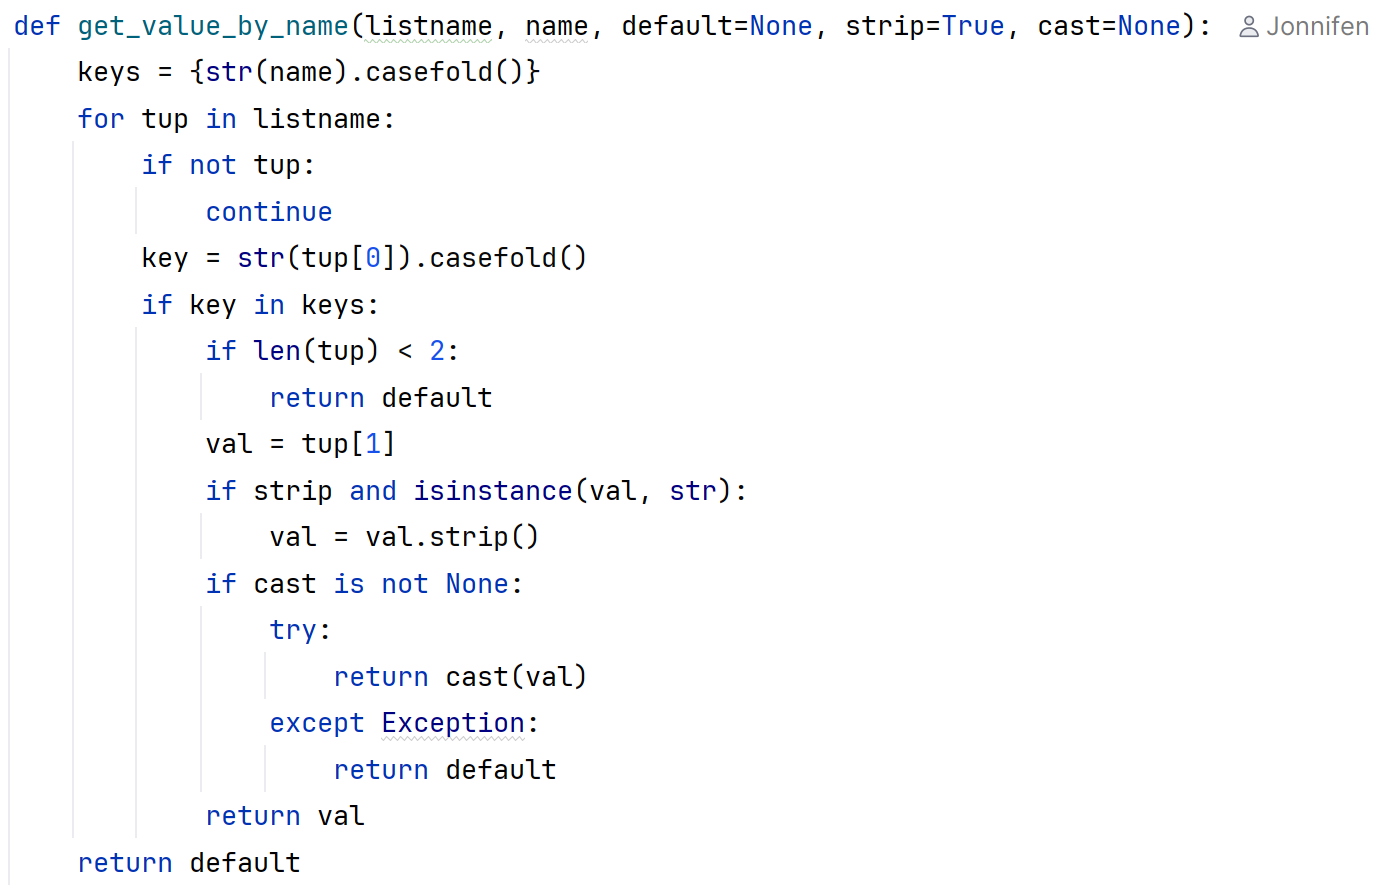
\includegraphics[width=1\textwidth]{Grafiken/get value by name}
    \caption{Codeausschnitt für die Suchfunktion in den Listen}
    \label{fig: Codeausschnitt für die Suchfunktion in den Listen}
    {Quelle: Eigene Darstellung}
\end{figure}

Die \ac{ORM}-Objekte werden durch die Funktionen \code{.session.add()} und \code{.session.flush()} schon in die Datenbank geschrieben,
um die automatisch generierten Primärschlüssel der Objekte erhalten zu können.
Die richtige Transaktion der \ac{ORM}-Objekte wird erst am Ende der Funktion \code{ingest\_xml()} ausgeführt, damit nur
vollständig einpflegbare XML-Daten in die Datenbank überführt werden können.
Bei einem Fehler werden alle Transaktionen rückgängig gemacht und die ausstehenden Änderungen gelöscht und es wird ein Fehler zurückgegeben.

Neben dieser Sicherung werden alle vermeintlichen Eintragungen bzw. \ac{ORM}-Objekte noch mal in der Datenbank über
Funktionen \code{execute()} und \code{select()} gesucht.
Wenn das Element bereits in der Datenbank existiert, wird es nicht eingefügt, um Dopplungen zu vermeiden. Ein Codebeispiel für
Die Sicherung ist in Abbildung \ref{fig: Beispiel ORM-Objekt} dargestellt.
Die Prüfungen sind in diesem Prototyp nicht identisch und können geringfügige Variationen beinhalten.

\begin{figure}[H]
    \centering
    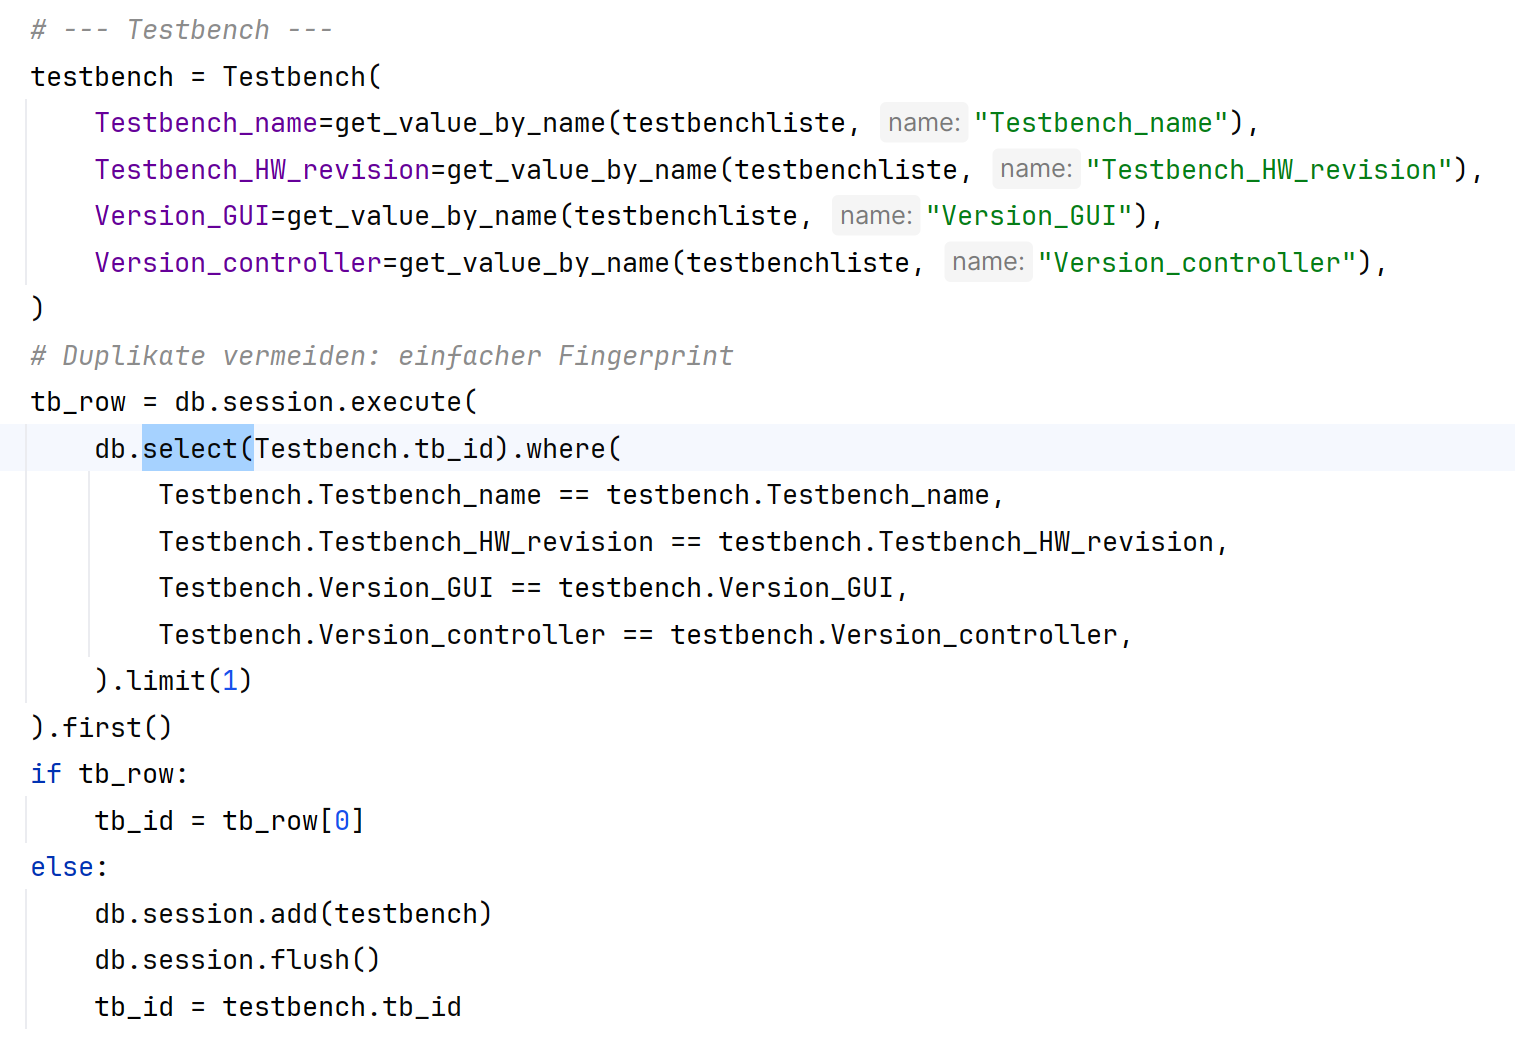
\includegraphics[width=1\textwidth]{Grafiken/Beispiel ORM Obj}
    \caption{Beispiel ORM-Objekt}
    \label{fig: Beispiel ORM-Objekt}
    {Quelle: Eigene Darstellung}
\end{figure}

Bei einem erfolgreichen Einfügen wird die Report-ID aus dem Eintrag aus der Datenbank an \code{upload()} zurückgegeben.
Diese erstellt dann eine Erfolgsnachricht, welche dann auf der Benutzeroberfläche der Seite ausgegeben wird.
In Abbildung \ref{fig: Code routes.py aus Upload-Seite} ist der Code aus der \code{routes.py} von der Upload-Seite dargestellt.

\begin{figure}[H]
    \centering
    \includegraphics[width=1\textwidth]{Grafiken/5.3.1}
    \caption{Code routes.py aus Upload-Seite}
    \label{fig: Code routes.py aus Upload-Seite}
    {Quelle: Eigene Darstellung}
\end{figure}








\subsection{Implementierung der Datenbank}
\label{subsec:implementierung-der-datenbank}


Die Datenbank wurde mithilfe von Flask-SQLAlchemy umgesetzt, das als ORM-Schicht die Kommunikation zwischen Anwendung und MariaDB realisiert. Grundlage des Datenmodells bildet das in Kapitel 4 entwickelte Entity-Relationship-Modell (ERM).


Die implementierten Tabellen umfassen Entitäten für:


\begin{itemize}

\item
Berichte (report)




\item
Testmodule (module)




\item
Prüfanlagen und Teststände (testbench)




\item
Messdaten (measurement)




\item
Parameter (parameter)




\item
DUTs (dut)




\end{itemize}

Über Fremdschlüsselbeziehungen werden die jeweiligen Abhängigkeiten zwischen den Entitäten abgebildet.

Die Datenbankanbindung erwies sich als stabil; Testeinträge konnten erfolgreich erstellt, abgefragt und gelöscht werden. Durch die Nutzung des ORM-Modells ist die Implementierung klar strukturiert und leicht wartbar.


Geplant ist eine Erweiterung der Datenbank um Benutzer- und Rollenmodelle, um künftig eine differenzierte Benutzerhierarchie (z. B. Administratoren, Standardnutzer, Gastzugänge) zu ermöglichen.



\subsection{Technischer Ablauf der Visualisierung}
\label{subsec:technische-details-zur-visualisierung}


Im folgenden Unterkapitel wird der Ablauf des Erstellens der Tabelle für die in der Datenbank enthaltenen Berichte, so wie die
Erstellung der Graphen grob beschrieben und ein Beispiel der Ergebnisse gegeben.

\subsubsection{Erstellen der Berichtstabelle}

Das Erstellen der Berichtstabelle für die Seite „Report-Tabelle“ läuft wie folgt ab:

\begin{enumerate}

    \item Beim Laden der Seite oder beim Bestätigen bzw. Zurücksetzen der Filterbedingungen wird die Funktion \code{report()} der Seite ausgeführt.
    Diese übermittelte die Filterinhalte über die GET-Methode an die Funktion \code{query_reports()} aus der Datei \code{queries.py}.
    Diese Funktion führt über \code{db} einen SELECT-Befehl über die Reportdaten aus, welche die Filterbedingungen erfüllen.
    \item Die ausgewählten Datensätze werden nach Rp\_id geordnet und an die Funktion \code{report()} aus der Route-Datei der Seite zurückgegeben.
    Die Datei \code{route.py} ist für die Veranschaulichung in Abbildung \ref{fig:Code routes.py aus Report-Tabellen-Seite} dargestellt.
    \item Diese Funktion lädt das Template der Seite neu und übergibt die ausgewählten Datensätze.
    \item Durch das erneute Laden wird mittels der HTML-Datei \code{reports.html} und der JavaScript-Datei \code{datatable.js} eine Tabelle mit den
    Ausgewählten Datensätzen erstellt.

\end{enumerate}

\begin{figure}[H]
    \centering
    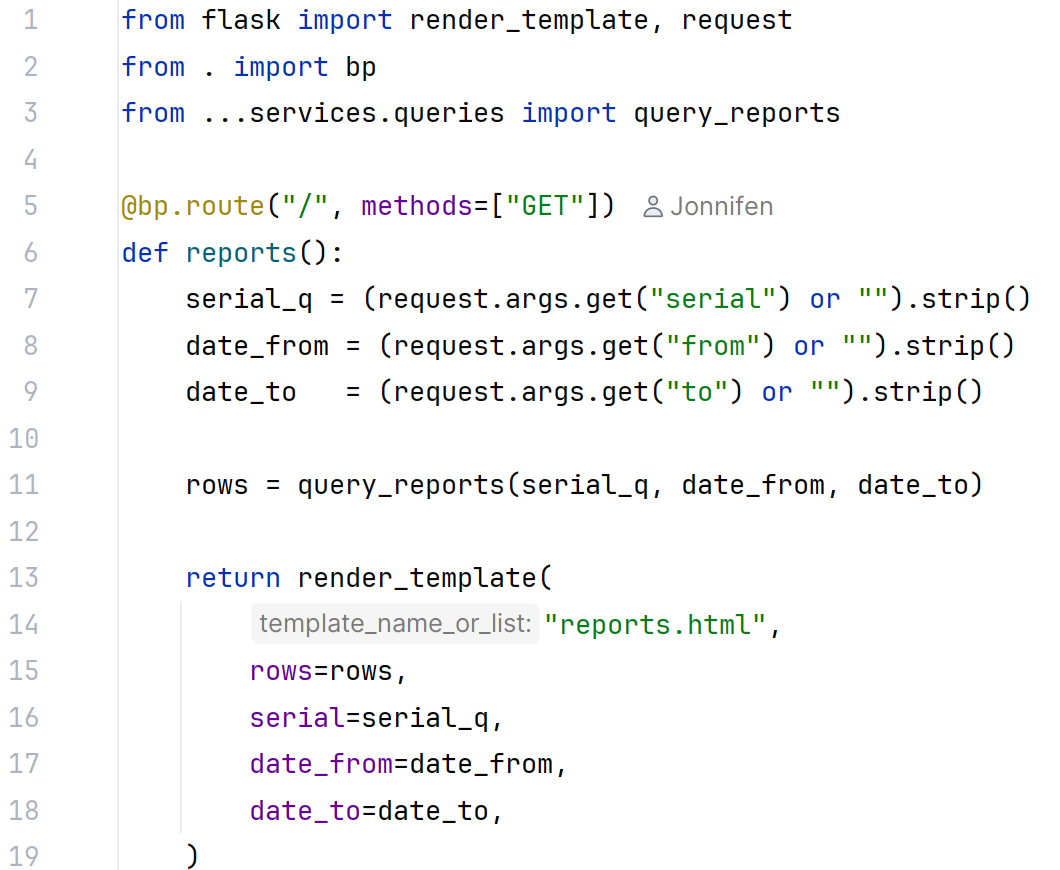
\includegraphics[width=1\textwidth]{Grafiken/route-reports}
    \caption{Code routes.py aus Report-Tabellen-Seite}
    \label{fig:Code routes.py aus Report-Tabellen-Seite}
    {Quelle: Eigene Darstellung}
\end{figure}

Dieser Ablauf wird jedes Mal, wenn die Seite geladen oder z. B. durch das Ändern der Filterbedingungen refreshed wird, durchgeführt.
Nach dem Laden der Seite für die Report-Tabelle werden erst alle in der Datenbank enthaltenen Berichte ausgegeben, bis Filterargumente festgelegt und bestätigt werden.
Ein Ausschnitt dieser Tabelle ist in Abbildung \ref{fig:Ausschnitt der Report-Tabelle} dargestellt.

\begin{figure}[H]
    \centering
    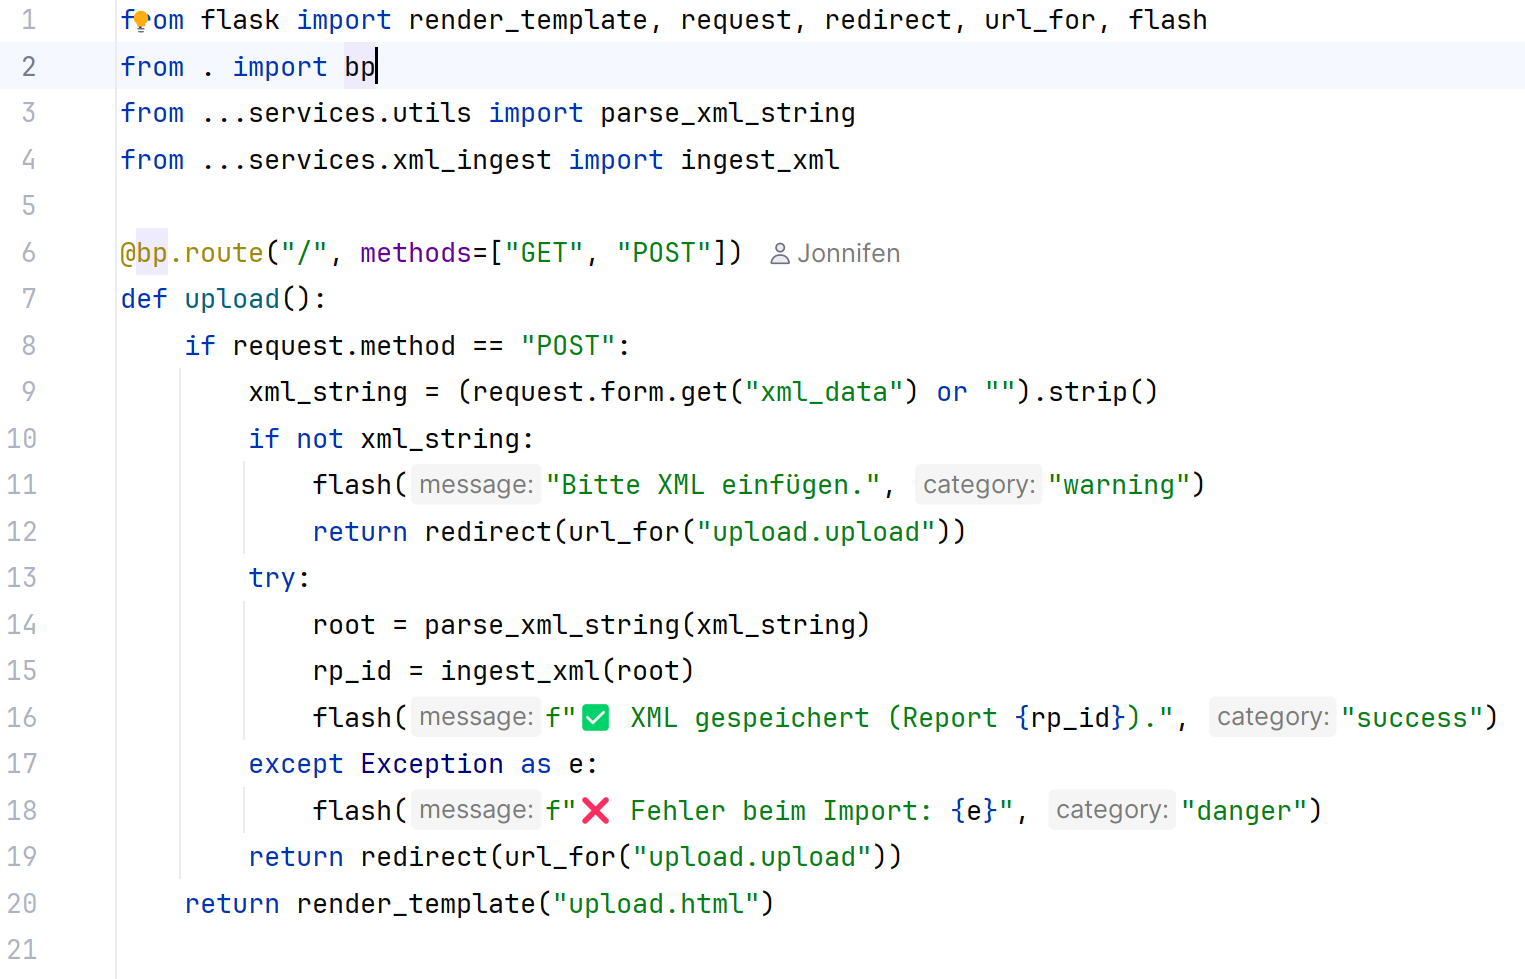
\includegraphics[width=1\textwidth]{Grafiken/Code route Up}
    \caption{Ausschnitt der Report-Tabelle}
    \label{fig:Ausschnitt der Report-Tabelle}
    {Quelle: Eigene Darstellung}
\end{figure}

\subsubsection{Erstellen der Messwert-Graphen}

Das Erstellen der Graphen ähnelt vom grundlegenden Ablauf her der Seite „Report-Tabelle“.
Der Ablauf für das Erstellen der Graphen der Analyse-Seite läuft wie folgt ab:

\begin{enumerate}

    \item Die Variablen zum Finden des gesuchten \ac{DUTs} können über das Eingeben der in die Suchfelder auf der Analyse-Seite
    oder über Links in der Tabelle auf der Seite der Report-Tabelle eingetragen werden.
    Das Laden dieser Variablen geschieht über die GET-Methode.
    und wird über die Funktion \code{dut\_root()} aus der Route-Datei für die Analyse-Seite durchgeführt.
    \item Die Funktion \code{dut\_root()} führt über \code{db} SELECT-Befehle aus, um die notwendigen Datensätze für die darzustellenden Testmodule (PulsTest und XPowerTest) zu erhalten.
    Hierfür werden Funktionen, unter anderem die Funktion \code{get\_series\_vals\_and\_unit()} aus \code{queries.py}, verwendet, um Datensätze zu suchen.
    Für eine Darstellung der Funktion siehe Abbildung \ref{fig:Beispielcode einer Such-Funktion}.
    \item Die ausgewählten Datensätze werden noch geordnet und am Ende lädt die Funktion die Seite neu.
    \item Beim Neuladen werden die Daten an die HTML-Datei \code{dut\_analyse.html} weitergegeben.
    In dieser werden die geordneten Datensätze mit Hilfe der JavaScript-Dateien \code{dut\_plot.js} und \code{plotly-latest.min.js} verarbeitet und die Graphen für die Analyse-Seite erstellt und ausgegeben.

\end{enumerate}

\begin{figure}[H]
    \centering
    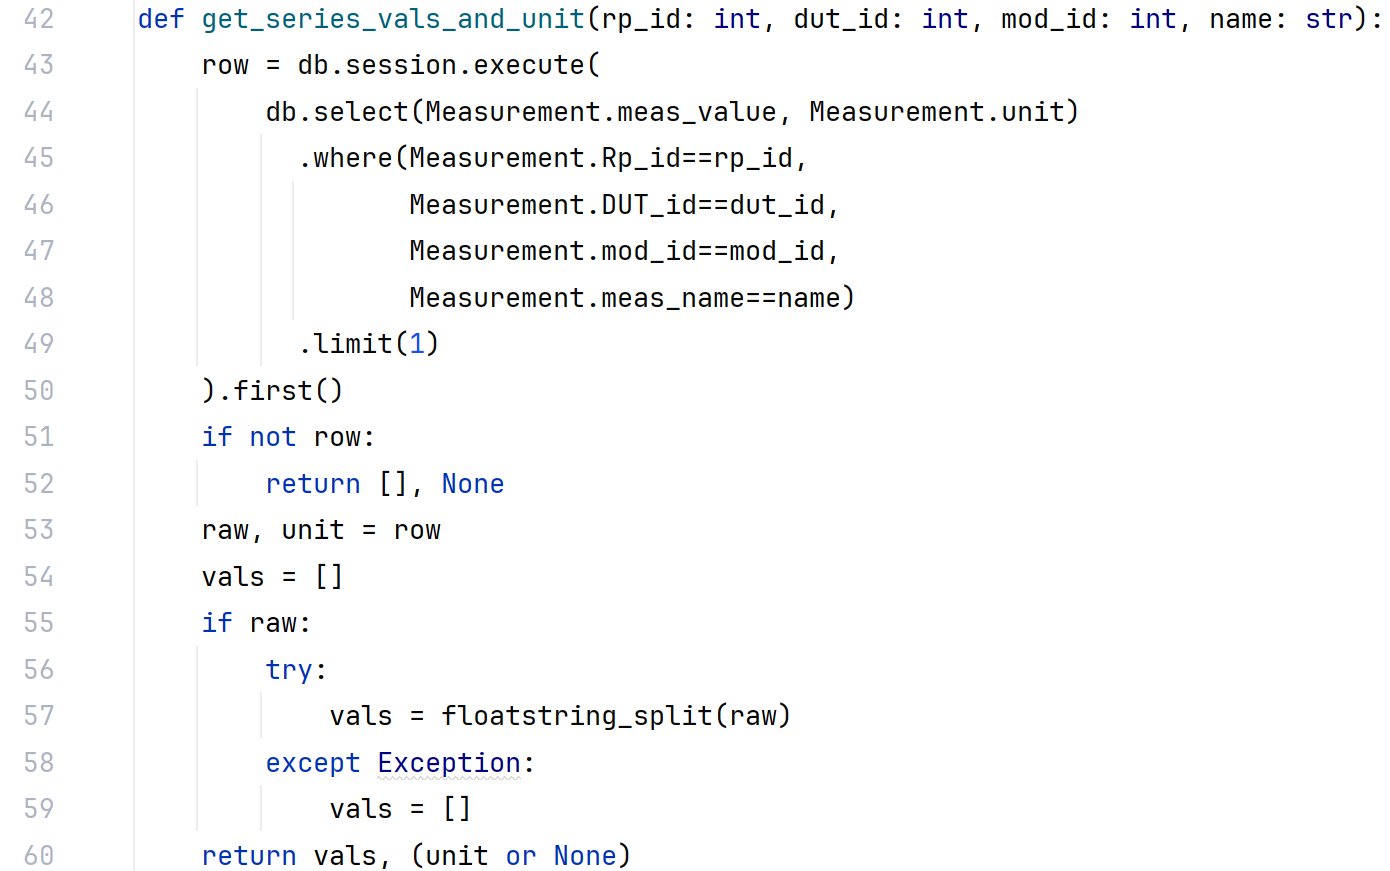
\includegraphics[width=1\textwidth]{Grafiken/get-series.png}
    \caption{Beispielcode einer Such-Funktion}
    \label{fig:Beispielcode einer Such-Funktion}
    {Quelle: Eigene Darstellung}
\end{figure}

Dieser Ablauf wird jedes Mal, wenn die Seite geladen oder z. B. durch das Ändern der Suchbedingungen refreshed wird, durchgeführt.
In der Folge sind zwei auf diese Weise erstellte Graphen dargestellt.
In Abbildung \ref{fig:Beispiel-Graph für PulsTest-Daten} ist ein Graph für die Darstellung der PulsTest-Daten dargestellt.
Die Abbildung \ref{fig:Beispiel-Graph für XPowerTest-Daten} ist ein Graph für die Darstellung der XPowerTest-Daten.

\begin{figure}[H]
    \centering
    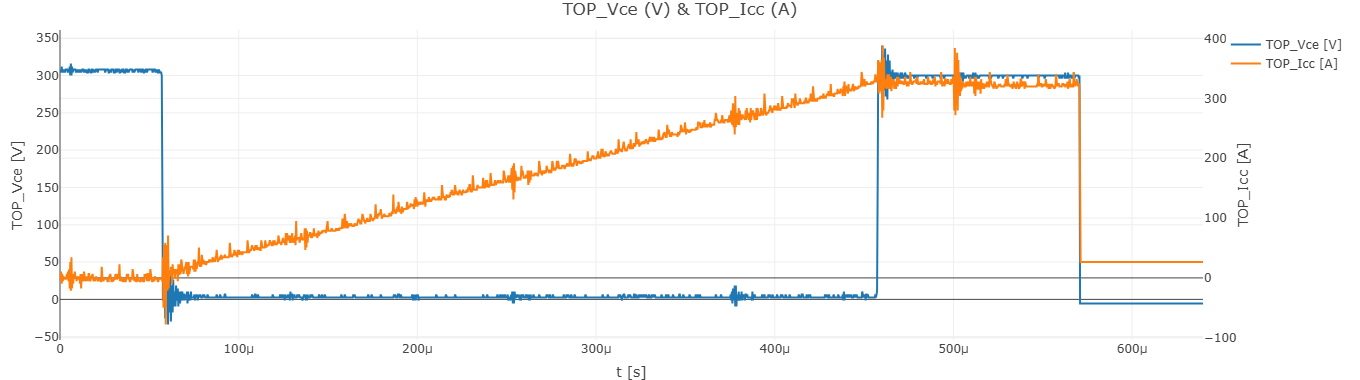
\includegraphics[width=1\textwidth]{Grafiken/newplot.png}
    \caption{Beispiel-Graph für PulsTest-Daten}
    \label{fig:Beispiel-Graph für PulsTest-Daten}
    {Quelle: Eigene Darstellung}
\end{figure}

\begin{figure}[H]
    \centering
    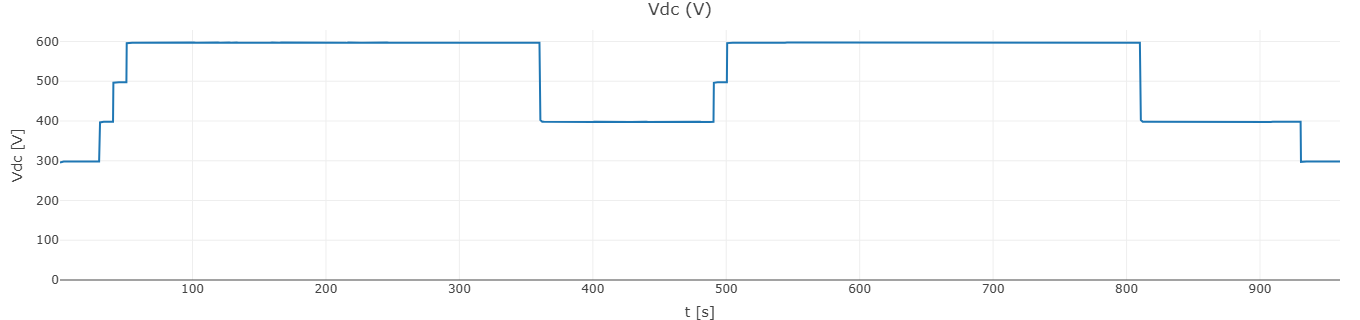
\includegraphics[width=1\textwidth]{Grafiken/newplot (1).png}
    \caption{Beispiel-Graph für XPowerTest-Daten}
    \label{fig:Beispiel-Graph für XPowerTest-Daten}
    {Quelle: Eigene Darstellung}
\end{figure}

Die auf diese Weise erstellten Graphen wurden mit den späteren Nutzern überarbeitet, um die fachgerechte Darstellung und Benennung der Graphen zu gewährleisten.


